
\begin{slikaDesno}{fig/fir.pdf}
    \PID У FIR филтру приказаном на слици употребљени су идеални блокови за кашњење, идеални множачи константом и идеални сабирачи.
    Одредити функцију преноса датог филтра $H(z)$ и одредити његов импулсни одзив $h[n]$.
    Скицирати његову амплитудску и фазну фреквенцијску карактеристику.        
\end{slikaDesno}
\textit{Помоћ:} Може се искористити резултат множења полинома $(1 + x + x^2)^2 = 1 + 2x + 3x^2 + 2x^3 + x^4$. 
%\begin{figure}[ht!]
%    \centering
%    \includegraphics
%\end{figure}

\RESENJE
Пратећи ток сигнала на блок дијаграму, функција преноса датог филтра је 
$H(z) = 1 + 2 z^{-1} + 3 z^{-2} +  2 z^{-3} + z^{-4}$. Његов импулсни одзив се одређује помоћу 
табличног пара \reft{T:ZT:delta} и правила о померању у временском домену па је 
$h[n] = \IZT{H(z)} = \updelta[n] + 2 \updelta[n-1] + 3\updelta[n-2] + 2\updelta[n-3] + \updelta[n-4]$. 
На основу дате напомене, може се писати $H(z) = (1 + z^{-1} + z^{-2})^2$, па се применом обрасца са суму 
геометријске прогресије\footnote{Сума која се користи је 
$\sum_{k = 0}^n q^k = \dfrac{1 - q^{n+1}}{1 - q}$, осим за  $k = 1$ када је сума једнака $(n+1)q$.
} добија 
\begin{eqnarray}
    H(z) = \left( \dfrac{1 - z^{-3}}{1 - z^{-1}} \right)^2 
\end{eqnarray}
Добијени облик се може поједноставити сређивањем до супротних експонената $z$, па затим преласком 
у облик $z = \uprho \ee^{\jj\Upomega}$, као
\begin{eqnarray}
    H(z) &=& 
    \left( \dfrac{ z^{-3/2} (z^{3/2} - z^{-3/2}) }{ z^{-1/2} (z^{1/2} - z^{-1/2})  } \right)^2
    =
    \left( z^{-1} \,\, \dfrac{ \cancel{\uprho} \, ( \ee^{\jj3\Upomega/2} - \ee^{-\jj3\Upomega/2} ) }{\cancel{\uprho}\,( \ee^{\jj\Upomega/2} - \ee^{-\jj\Upomega/2} )} \right)^2
    \\
    &=&
    \left(
        z^{-1}
        \dfrac{\sin(3\Omega/2)}{\sin(\Omega/2)}
    \right)^2
    =
    \left(\dfrac{1}{\uprho}\right)^2 \ee^{-\jj 2\Upomega} 
    \left(
        \dfrac{\sin(3\Omega/2)}{\sin(\Omega/2)}
    \right)^2
\end{eqnarray}
Амплитудска и фазна фреквенцијска карактеристика траже се у случају када је $z = \ee^{\jj\Omega}$, односно на јединичној
кружници $\uprho = 1$ па је 
\begin{eqnarray}
    H(\ee^{\jj\Omega}) = 
    \underbrace{
    \left(
        \dfrac{\sin(3\Omega/2)}{\sin(\Omega/2)}
    \right)^2
    }_{|H(\ee^{\jj\Omega})|}
    \exp\left(\jj 
    \underbrace{-2\Upomega}_{
        \arg H(\ee^{\jj\Omega})
    } \right)
\end{eqnarray}

Добијена амплитудска и фазна фреквенцијска карактеристика приказане су на слици \ref{fig:\ID.hz}
\begin{figure}
    \centering
    \begin{subfigure}{0.49\textwidth}
        \centering
        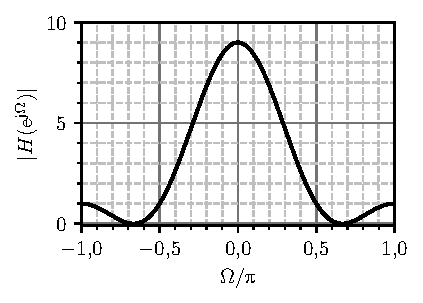
\includegraphics{fig/zt_tri.pdf}
    \end{subfigure}
    %
    \begin{subfigure}{0.49\textwidth}
        \centering
        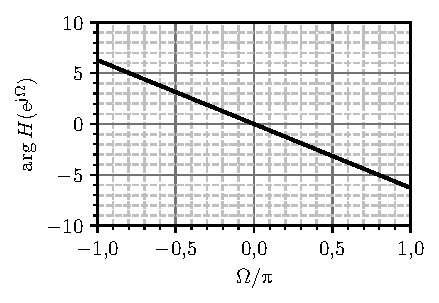
\includegraphics{fig/zt_tri_faz.pdf}
    \end{subfigure}
    \caption{Тражене амплитудска односно фазна карактеристика филтра.}
    \label{fig:\ID.hz}
\end{figure}

Добијени резултат одговара квадрату Дирихлеове функције, из задатка \refz{dtft_rec}, што није случајност. 
Такав резултат последица је чињенице да се импулсни одзив датог филтра може представити и као 
конволуција два правоугаона прозора $h[n] = \rect_1[n] \ast \rect_1[n]$. Због тога, функција преноса 
разматраног филтра једнака је квадрату функције преноса 
филтра чији је импулсни одзив правоугаони прозор. Случајност није ни појава множења полинома, будући да множење полинома само по 
себи представља дискретну конволуцију њихових коефицијената, како је показано у задатку \refz{konv_pol_pol}
